%!TEX root = theory.tex
% =========================================================================
% -------------------------------------------------------------------------
% Single and Multiphase Flow:
% -------------------------------------------
%
%  This is a good place to outline key objectives of this section.
%
% -------------------------------------------------------------------------

% bold symbols
\def\bnabla{{\boldsymbol{\nabla}}}
\def\bg{{\boldsymbol{g}}}
\def\bq{{\boldsymbol{q}}}
\def\bx{{\boldsymbol{x}}}
\def\bJ{{\boldsymbol{J}}}
\def\K{{\mathbb K}}

% abbreviations
\def\Frac{\displaystyle \frac}

% units
\def\ucdot{{\,\cdot\,}}
\def\ukg{{\rm kg}}
\def\um{{\rm m}}
\def\us{{\rm s}}
\def\umol{{\rm mol}}
\def\upa{{\rm Pa}}

\section{Flow Processes}         
\label{sec:flow-processes}

\subsection{Overview}

Subsurface flow simulations typically assume that Darcy's law is
valid. As this law gives a relationship between velocity and pressure,
it essentially replaces the momentum equation. There has been much
research to support the validity of Darcy's
Law~\citep{bear-1972}.
Most references give the applicability of
Darcy's Law to be for laminar flows with Reynolds numbers less that 10 using the pore throat diameter for a soil.
There has been some effort to include inertial as well as turbulence effects that can occur near the wells.

It is also assumed that thermodynamic equilibrium (mechanical and
thermal) exists for each grid block.  Sub-grid scale features will
often play a prominent role in multi-fluid simulations. Faults and
fractures will likely be fast paths for contaminant transport and can
effectively be treated with multiple porosity models. Similarly,
rate-limited diffusion from clay inclusions can also be modeled with a
multiple porosity material.

\begin{center}
\begin{longtable}{cp{7cm}c}
\caption{List of local variables.} \label{table:flow-list-of-variables} \\

\multicolumn{1}{c}{Symbol} & \multicolumn{1}{c}{Meaning} & \multicolumn{1}{c}{Units} \\
\hline  \hline 
\endfirsthead

\multicolumn{3}{c}{{\tablename} \thetable{} -- Continued} \\
\multicolumn{1}{c}{Symbol} & \multicolumn{1}{c}{Meaning} & \multicolumn{1}{c}{Units} \\
\hline  \hline 
\endhead

\hline \multicolumn{3}{c}{{Continued on next page}} \\ 
\hline \hline 
\endfoot

\hline \hline
\endlastfoot

$\bg$      & gravity vector       &  $\um\ucdot\us^{-2}$  \\
$g$        & gravity magnitude    &  $\um\ucdot\us^{-2}$  \\
$\K$       & absolute permeability tensor & $\um^2$ \\
$k_{rl}$   & relative permeability&  $-$ \\
$p_l$      & liquid pressure      &  $\upa$ \\
$\bq$      & Darcy velocity       &  $\um\ucdot\us^{-1}$  \\
$S_s$      & specific storage     &  $\um^{-1}$  \\
$S_y$      & specific yield       &  $-$  \\
$s_l$      & liquid saturation    &  $-$ \\
$\mu_l$    & liquid viscosity     &  $\upa\ucdot\us$ \\
$\rho_l$   & liquid density       &  $\ukg\ucdot\um^{-3}$ \\
$\phi$     & porosity             &  $-$  \\
$\phi_f$   & porosity of fracture &  $-$  \\
$\phi_m$   & porosity of matrix   &  $-$  \\
$\eta_l$   & molar liquid density &  $\umol\ucdot\um^{-3}$ \\
$\theta$   & volumetric water content  &  $\umol\ucdot\um^{-3}$ \\
$\theta_f$ & volumetric water content of fracture &  $\umol\ucdot\um^{-3}$ \\
$\theta_m$ & volumetric water content of matrix   &  $\umol\ucdot\um^{-3}$ \\

\end{longtable}
\end{center}


%%%%%%%%%%%%%%%%%%%%%%%%%%%%%%%%%%%%%%%%%%%%%%%%%%%%%%%%%%%%%%%%%%%%%%%%%%%%%%%%%%%%
%%%%%%%%%%%%%%%%%%%%%%%%%%%%%%%%%%%%%%%%%%%%%%%%%%%%%%%%%%%%%%%%%%%%%%%%%%%%%%%%%%%%

\subsection{Single-Phase Flow}
\label{sec:flow-single-phase}

The most basic flow model is a single-phase flow in a porous medium.  
Notwithstanding its simplicity, it has a wide application to
describing subsurface processes.


%%%%%%%%%%%%%%%%%%%%%%%%%%%%%%%%%%%%%%%%%%%%%%%%%%%%%%%%%%%%%%%%%%%%%%%%%%%%%%%%%%%%
\subsubsection{Assumptions and Applicability}

There are many assumptions required for the strict validity of Darcy's
Law, including incompressible and laminar flow.
We also assume that rock is incompressible and fluid viscosity is constant.


%%%%%%%%%%%%%%%%%%%%%%%%%%%%%%%%%%%%%%%%%%%%%%%%%%%%%%%%%%%%%%%%%%%%%%%%%%%%%%%%%%%%
\subsubsection{Process Model Equations}

The governing equations for the single phase flow in porous media 
under isothermal conditions are
\begin{equation}
  \phi \left(\Frac{S_s}{g} + \Frac{S_y}{L\,g}\right) \frac{\partial p_l}{\partial t} 
  =
  \boldsymbol{\nabla} \cdot (\rho_l \boldsymbol{q}_l) + Q,
  \qquad
  \bq_l = -\frac{\K}{\mu_l} 
  (\bnabla p_l - \rho_l \bg),
\end{equation}
where $L$ is a characteristic size of the yield layer, and 
$Q$ is source or sink term [$\ukg \ucdot \um^{-3} \ucdot \us^{-1}$].
It is common to see the Darcy Law written in terms of hydraulic head $h$ [$\um$]
and the hydraulic conductivity tensor $\K_h$:
\begin{equation}  \label{eq:HydraulicHead}
  \bq = -\K_h \bnabla h,\quad
  h \eq  z + \frac{p_l}{\rho_l g},\quad
  \K_h = \K \frac{\rho_l g}{\mu_l}.
\end{equation}

Three types of boundary conditions are supported by the model:
1) prescribed pressure (or head);
2) prescribed flux;
3) semipervious boundary \citep[for reference see][]{bear-1979}.
These boundary conditions are described in Section~\ref{sec:flow-boundary-conditions}.


%%%%%%%%%%%%%%%%%%%%%%%%%%%%%%%%%%%%%%%%%%%%%%%%%%%%%%%%%%%%%%%%%%%%%%%%%%%%%%%%%%%%
%%%%%%%%%%%%%%%%%%%%%%%%%%%%%%%%%%%%%%%%%%%%%%%%%%%%%%%%%%%%%%%%%%%%%%%%%%%%%%%%%%%%

\subsection{Isothermal Richards Equation}
\label{sec:richards-equation}

The Richards equation is often used to describe single phase flow under partially 
saturated conditions (i.e., the pores are not occupied exclusively by a single phase).  
As such, it requires the introduction of a relative permeability and a capillary 
pressure relations as discussed in Section~\ref{sec:pc_s_relations}.
The Richards equation is well suited to very large numerical problems (millions of 
degrees of freedom) because it requires only one independent variable per cell.


%%%%%%%%%%%%%%%%%%%%%%%%%%%%%%%%%%%%%%%%%%%%%%%%%%%%%%%%%%%%%%%%%%%%%%%%%%%%%%%%%%%%
\subsubsection{Assumptions and Applicability}

The Richards equation makes the fundamental assumption that we are neglecting
the movement of the gas phase.
Because of this assumption, using the Richards equation may limit the kinds of 
transport analysis that can be done.
It should also be noted that the Richards equation is often highly nonlinear
due to strong dependence of the relative permeability of the liquid phase
on the liquid saturation.


%%%%%%%%%%%%%%%%%%%%%%%%%%%%%%%%%%%%%%%%%%%%%%%%%%%%%%%%%%%%%%%%%%%%%%%%%%%%%%%%%%%%
\subsubsection{Process Model Equations} 
\label{sec:richards-model-equations}

The Richards equation is derived from the conservation of
liquid mass continuity equation.
In the mixed formulation, this equation is continuous when 
transitioning from the saturated zone to the vadoze zone:
\begin{equation}
  \frac{\partial \theta}{\partial t} 
  = \bnabla \cdot (\eta_l \bq_l) + Q,
  \qquad
  \bq_l = -\frac{\K k_{rl}}{\mu_l} 
  (\bnabla p_l - \rho_l \bg),
\end{equation}
where $Q$ is source or sink term [$\ukg \ucdot \um^{-3} \ucdot \us^{-1}$].
Usage of the molar liquid density allows us to extend easily the model to a non-isothermal case.
The total volumetric water content is defined as
$$
  \theta = \phi\, \eta_l\, s_l.
$$
Porosity is in general a function of pressure.

The primary dependent variable is liquid pressure $p_l$.
Recall that the relative permeability is the function of saturation $s_l$
which in turns is a function of capillary pressure $p_c$. 
Typical models of relative permeability are the van Genuchten-Mualem relations \eqref{eq:krl_vGM}
and the Brooks-Corey-Burdine relations \eqref{eq:krl_BCB}.

Four types of boundary conditions are supported by the model:
1) prescribed pressure (or head);
2) prescribed flux;
3) semipervious boundary \citep[for reference see][]{bear-1979};
4) seepage face.
These boundary conditions are described in Section~\ref{sec:flow-boundary-conditions}.


%%%%%%%%%%%%%%%%%%%%%%%%%%%%%%%%%%%%%%%%%%%%%%%%%%%%%%%%%%%%%%%%%%%%%%%%%%%%%%%%%%%%
\subsubsection{Capillary Pressure -- Saturation Relations}  
\label{sec:richards-pc_s_relations}

Richards equation for unsaturated flow, as well as more general
multiphase flow models, require representations of the capillary
pressure and the relative permeability.  The capillary pressure is a
fundamental dependent variable in the multi-phase flow model, and
relates the difference in pressure across an interface between two
fluids to the tendency of a porous medium to pull in the wetting fluid
and push out the non-wetting fluid.
For the two-phase fluid flow model typically used to
characterize air-water systems, there is only a single capillary pressure,
\begin{equation} \label{eq:GasLiquidCapillaryPressure}
  p_c = p_g - p_l
\end{equation}
where $p_g$ is the pressure of the air. 
Let us define the effective liquid saturation $s_e$ as
\begin{equation}
\label{eq:SaturationDefinition}
s_e \eq \frac{s_l^{} - s_l^r}{s_l^0 - s_l^r}, 
\end{equation}
where $s_l^r$ is residual liquid saturation, and $s_l^0$ is the maximum liquid saturation.
Using these definitions, two widely
used capillary pressure-saturation relations, namely the van Genuchten
\citep{van1980closed} and Brooks-Corey \citep{brooks1964hydraulic} are
presented below.


\paragraph{Van Genuchten model.}
In the \citet{van1980closed} model the effective liquid saturation is
described by the relation
%
\begin{equation}  
  \label{eq:vG_s_pc_relation}
  s_e \eq \left[1+\left( \alpha |p_c| \right)^n \right]^{-m}, 
\end{equation}
%
with inverse relation
\begin{equation}
  \label{eq:vG_pc_s_relation}
  p_c \eq \frac{1}{\alpha} \left[ s_e^{-1/m} -1 \right]^{1/n}.
\end{equation}
%
The constants $n$ [-], $m$ [-] and $\alpha$ [$\upa^{-1}$] are
empirical parameters.


\paragraph{Brooks-Corey model.}
The Brooks-Corey form of the saturation function \citep{brooks1964hydraulic} is given by
\begin{equation}
  \label{eq:BC_s_pc_relation}
  s_e \eq \left( \alpha |p_c| \right)^{-\lambda}, 
\end{equation}
where $\lambda$ [-], and $\alpha$ [$\upa^{-1}$] are empirical parameters fit to experimental
observations.
The inverse relation is written,
\begin{equation}
  \label{eq:BC_pc_s_relation}
  p_c \eq \frac{1}{\alpha} s_e^{-1/\lambda}.
\end{equation}
Note that if $\lambda = mn$ and
$(\alpha p_c)^n \gg 1$, then the Brooks-Corey and van Genuchten
saturation functions, Equations \eqref{eq:BC_s_pc_relation} and
\eqref{eq:vG_s_pc_relation}, are equivalent.


%%%%%%%%%%%%%%%%%%%%%%%%%%%%%%%%%%%%%%%%%%%%%%%%%%%%%%%%%%%%%%%%%%%%%%%%%%%%%%%%%%%%
\subsubsection{Relative Permeability -- Saturation Relations}
\label{sec:richards-relative-permeability}

Given capillary pressure - saturation relations, the relative
permeability relations needed by Richards equation can be defined.  
Two popular relative permeability - saturation relations used in air-water 
systems are the \citet{mualem1976new} and \citet{burdine1953relative} models.
The relative permeability model proposed by \citet{mualem1976new} has the form
\begin{equation} \label{eq:Mualem}
  k_{rl}(s_l) = s_e^{\ell} \, 
    \frac{ \left\{ \displaystyle\int_0^{s_e} p_c(s)^{-1} ds \right\}^2 }
    { \left\{ \displaystyle\int_0^{1} p_c(s)^{-1} ds \right\}^2 },
\end{equation}
where $\ell$ is a pore-connectivity parameter that varies between soils. 
Although, \citet{mualem1976new} estimated an average value of
$\ell=1/2$, values of $\ell$ ranged from -5 to +5 across soils. More recent studies
[cf. \citet{vanG_retc_1991}] have suggested that $\ell=1/2$ may be
appropriate for coarse-textured soils, but not for many medium- and
fine-textured soils. Thus, $\ell$ should be available as a fitting parameter.
Similarly, the \citet{burdine1953relative} model is given by
\begin{equation}
\label{eq:Burdine}
  k_{rl}(s_l) = s_e^{\ell} \, 
    \frac{ \displaystyle\int_0^{s_e} p_c(s)^{-2} ds }
         { \displaystyle\int_0^{1} p_c(s)^{-2} ds },
\end{equation}
where \citet{burdine1953relative} assumed $\ell=2$. However, as with
the Mualem model \eqref{eq:Mualem}, $\ell$, should be available as a
fitting parameter.


\paragraph{Van Genuchten relative permeability.}
To obtain a closed-form solution for the relative permeability using
either the Mualem or Burdine models (Eqns.\eqref{eq:Mualem} and
\eqref{eq:Burdine}, respectively) combined with the van Genuchten
saturation function, the parameters $n$ and $m$ must be related by the
expressions
\begin{equation}
\label{eq:lambda} 
m = \left\{
  \begin{array}{ll}
    1 - \dfrac{1}{n}, & \text{Mualem},\\[9pt]
    1 - \dfrac{2}{n}, & \text{Burdine}.
  \end{array}
\right.
\end{equation}
In the more general case of independent values of $m$ and $n$ the
relative permeability involves the incomplete beta function \citep{vangenuchten1985}. 
More recently \citep{douradoneto2011} presented a general model for Mualem and 
Burdine relative permeability functions for use with the van Genuchten saturation 
function in terms of hypergeometric functions.

The Mualem relative permeability function for the liquid phase derived
from the van Genuchten saturation function is given by
\begin{equation}
  k_{rl} \eq s_e^{\ell} \left\{ 1 - \left[ 1 - s_e^{1/m} \right]^m \right\}^2.
  \label{eq:krl_vGM} 
\end{equation}
The Burdine relative permeability function has the form
\begin{equation}
  k_{rl} \eq s_e^{\ell} \left\{ 1 - \left[ 1 - s_e^{1/m} \right]^m \right\}.
  \label{eq:krl_vGB} 
\end{equation}


\paragraph{Brooks-Corey relative permeability.}
Combined with the Brooks-Corey saturation function, the Mualem
relative permeability function is given by
\begin{equation} \label{eq:krl_BCM}
  k_{rl} = \big(s_e\big)^{\ell+2+2/\lambda} 
         = \left(\alpha |p_c|\right)^{-((\ell+2)\lambda+2)}.
\end{equation}
The Burdine form originally considered by \citet{brooks1964hydraulic}
is given by
\begin{equation} \label{eq:krl_BCB}
  k_{rl} = \left( s_e \right)^{ \ell+1+2/\lambda}
         = \left( \alpha |p_c| \right)^{-((\ell+1)\lambda+2)}.
\end{equation}


%%%%%%%%%%%%%%%%%%%%%%%%%%%%%%%%%%%%%%%%%%%%%%%%%%%%%%%%%%%%%%%%%%%%%%%%%%%%%%%%%%%%
%%%%%%%%%%%%%%%%%%%%%%%%%%%%%%%%%%%%%%%%%%%%%%%%%%%%%%%%%%%%%%%%%%%%%%%%%%%%%%%%%%%%
\subsection{Thermal Richards Equation}
\label{sec:thermal-richards-equation}


%%%%%%%%%%%%%%%%%%%%%%%%%%%%%%%%%%%%%%%%%%%%%%%%%%%%%%%%%%%%%%%%%%%%%%%%%%%%%%%%%%%%
\subsubsection{Process Model Equations} 

\begin{equation}
  \frac{\partial \theta}{\partial t} 
  =
  \bnabla \cdot (\eta_l \bq_l)
  - \bnabla \cdot (\K_g \bnabla \big(\frac{p_v}{p_g}\big)) + Q,
  \qquad
  \bq_l = -\frac{\K k_r}{\mu} (\bnabla p - \rho_l \bg)
\end{equation}


%%%%%%%%%%%%%%%%%%%%%%%%%%%%%%%%%%%%%%%%%%%%%%%%%%%%%%%%%%%%%%%%%%%%%%%%%%%%%%%%%%%%
%%%%%%%%%%%%%%%%%%%%%%%%%%%%%%%%%%%%%%%%%%%%%%%%%%%%%%%%%%%%%%%%%%%%%%%%%%%%%%%%%%%%
\subsection{Isothermal Richards Equation with Dual Porosity Model}
\label{sec:dual-porosity-richards-equation}

Dual-porosity model assumes that water flow is restricted to the fractures and the
water in the matrix does not move.
The rock matrix represents immobile pockets that can exchange, retain and store water
but do not permit convective flow.
This leads to dual-porosity type flow and transport models that partition the liquid
phase into mobile and immobile regions.


%%%%%%%%%%%%%%%%%%%%%%%%%%%%%%%%%%%%%%%%%%%%%%%%%%%%%%%%%%%%%%%%%%%%%%%%%%%%%%%%%%%%
\subsubsection{Process Model Equations} 

The Richards equation in the mobile region is augmented by the water exchange
term $\Sigma_w$: 
\begin{equation}
  \frac{\partial \theta_f}{\partial t} 
  = \bnabla \cdot (\eta_l \bq_l) - \Sigma_w + Q_f,
  \qquad
  \bq_l = -\frac{\K k_r}{\mu} (\bnabla p_l - \rho_l \bg),
\end{equation}
where $\Sigma_w$ is transfer rate for water from the matrix to the fracture, 
and $Q_f$ is source or sink term [$\ukg \ucdot \um^{-3} \ucdot \us^{-1}$].
The equation for water balance in the matrix is
$$
  \frac{\partial \theta_m}{\partial t} 
  = Q_m + \Sigma_w,
$$
where and $Q_m$ is source or sink term [$\ukg \ucdot \um^{-3} \ucdot \us^{-1}$].
The volumetric volumetric water contents are defined as
$$
  \theta_f = \phi_f\, \eta_l\, s_{lf},\quad
  \theta_m = \phi_m\, \eta_l\, s_{lm},
$$
where saturations $s_{lf}$ and $s_{lm}$ may use different capillary pressure - saturation
models.
The rate of water exchange between the fracture and matrix regions is
proportional to the difference in hydraulic heads:
$$
  \Sigma_w = \alpha_w (h_f - h_m),
$$
where $\alpha_w$ is the mass transfer coefficient.
Since hydraulic heads are needed for both regions, this equation requires
estimating retention curves for both regions and therefore is nonlinear.


%%%%%%%%%%%%%%%%%%%%%%%%%%%%%%%%%%%%%%%%%%%%%%%%%%%%%%%%%%%%%%%%%%%%%%%%%%%%%%%%%%%%
%%%%%%%%%%%%%%%%%%%%%%%%%%%%%%%%%%%%%%%%%%%%%%%%%%%%%%%%%%%%%%%%%%%%%%%%%%%%%%%%%%%%
\subsection{Boundary conditions}
\label{sec:flow-boundary-conditions}


To facilitate the discussion on boundary conditions, consider the case of 
flow described in Fig.~\ref{fig:bc_flow}. 
Although the figure represents a two-dimensional flow field, the passage to three dimensions 
is straightforward and requires no further explanations. 

\begin{figure}  [h]
\begin{center} 
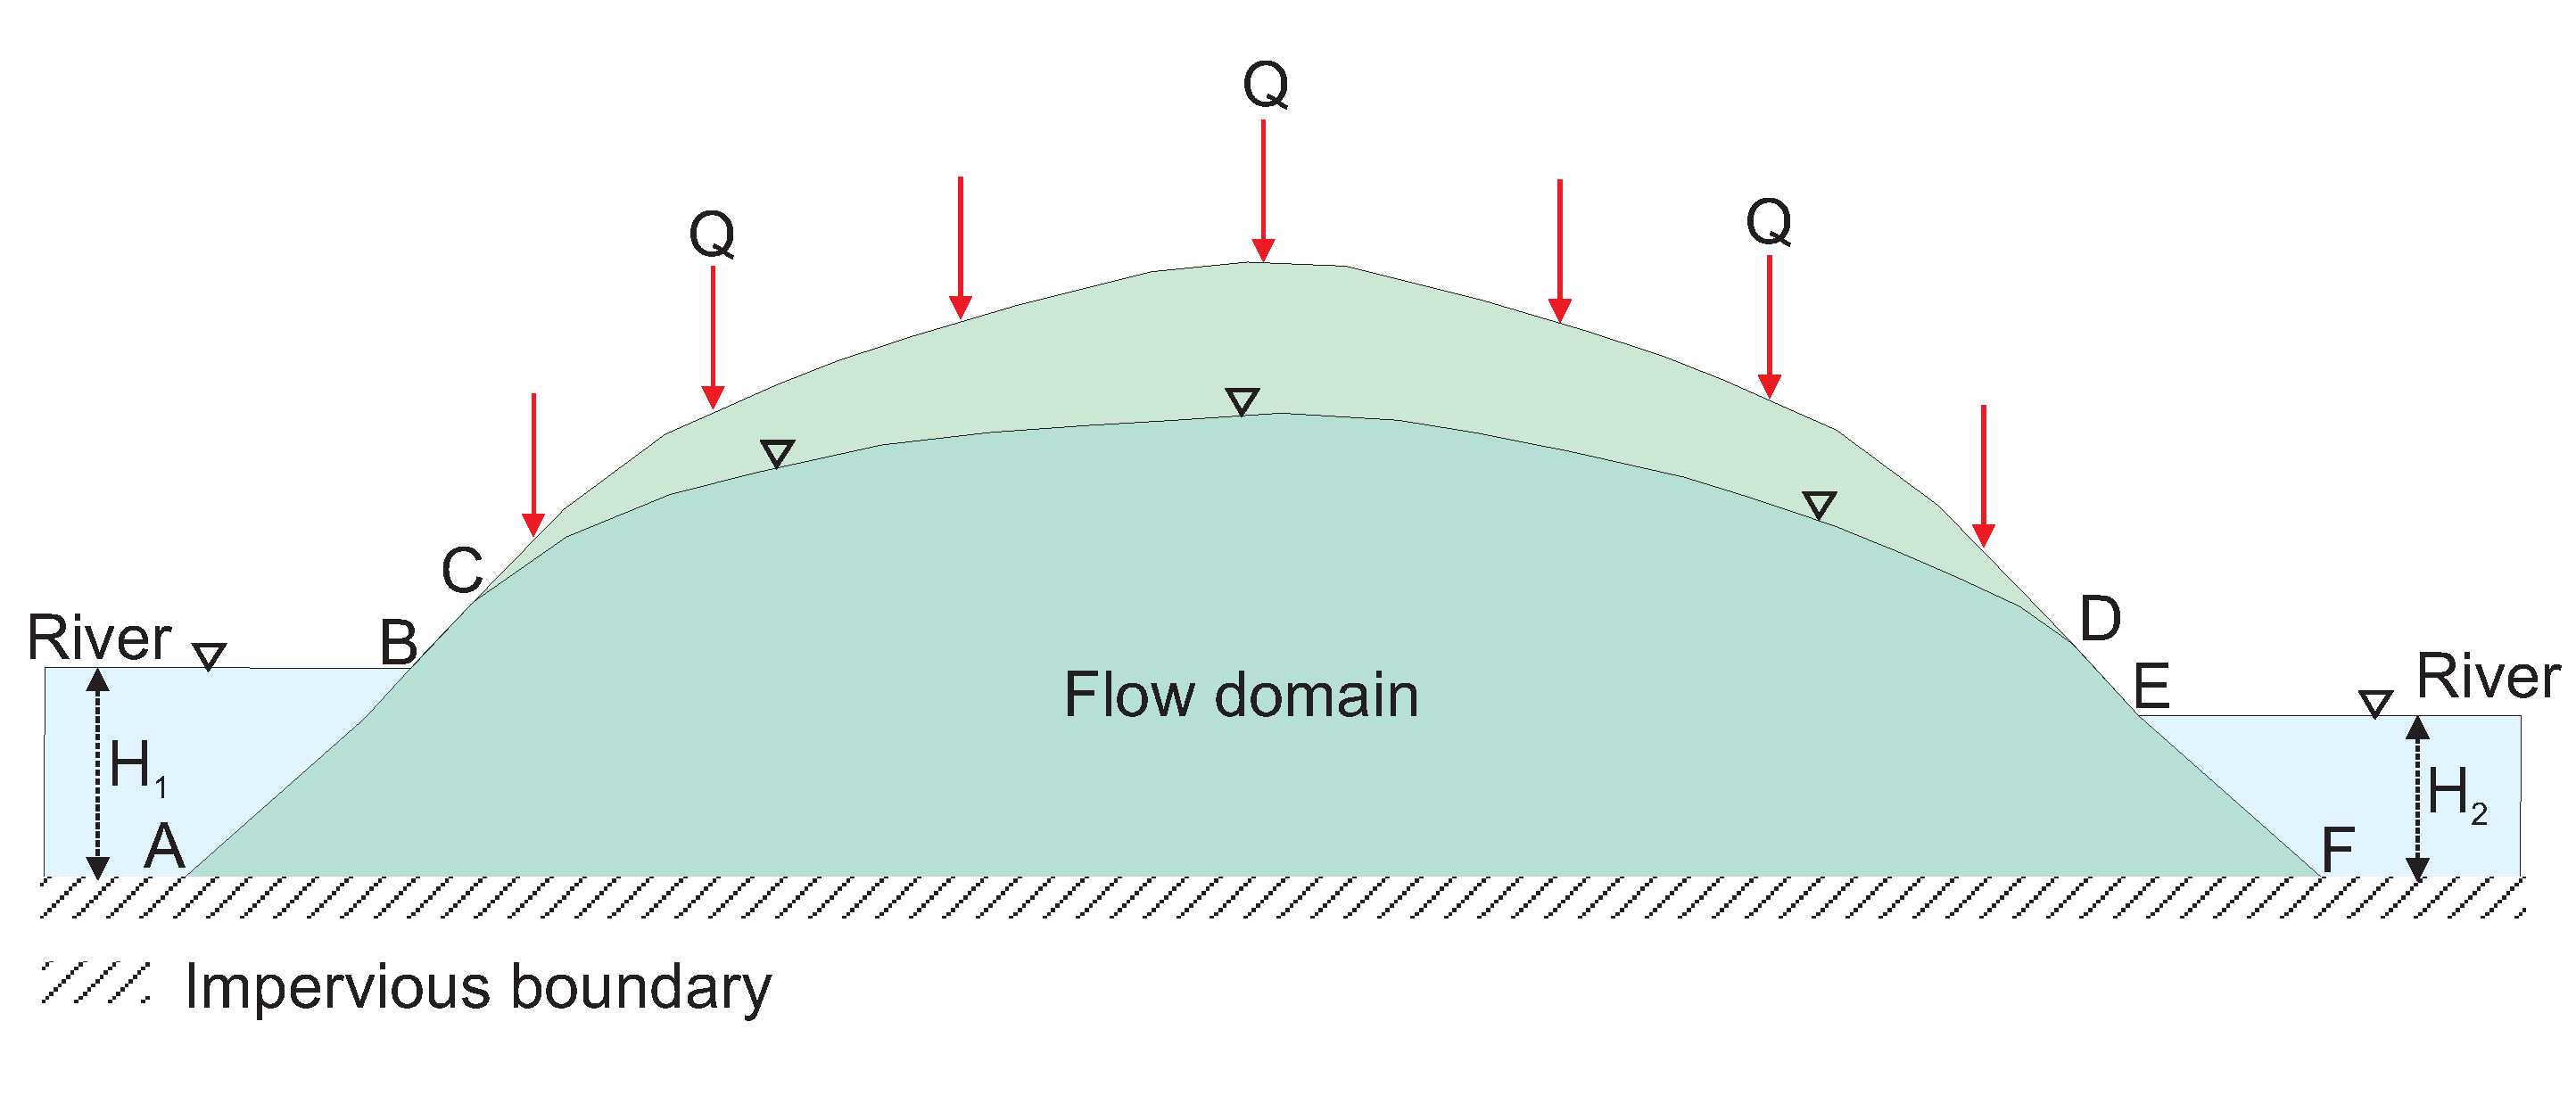
\includegraphics[scale=0.25]{bc_flow.pdf}
\caption{Flow domain between two rivers \citep[it was partially based on][Figure 5-7]{bear-1979}.}
\label{fig:bc_flow}
\end{center}
\end{figure}

\paragraph{Boundary of prescribed pressure or head.}
This involves the specification of a fixed pressure or hydrostatic head on boundary $\Gamma_D$.
For instance, a boundary of this kind occurs whenever the flow domain is adjacent to a body of open water.
Segments A-B and E-F in Fig.~\ref{fig:bc_flow} are examples of a boundary of prescribed potential.
The pressure or head boundary conditions are given functions, e.g.
\begin{equation}
  p_l(\bx,t) = p_{b}(\bx,t), \quad \bx \in \Gamma_D. 
\end{equation}

\paragraph{Boundary of prescribed flux.}
This involves the specification of the flux normal to the boundary $\Gamma_N$
(see segment C-D in Figure \ref{fig:bc_flow}):
\begin{equation}
  \bq_l\cdot \bn = q_{b}(\bx,t), \quad \bx \in \Gamma_N,
\end{equation}
where $q_b$ [$\um\ucdot\us^{-1}$] is the given boundary flux. 
For infiltration at the top horizontal surface, it equals to the Darcy velocity
and referred to as the infiltration velocity.

\paragraph{Semipervious boundary (or mixed boundary condition).}
This boundary condition is more complicated than the first two as it involves a case 
in which local conditions within the computational domain influence the flux in or 
out of the domain.
This type of boundary occurs when the porous medium domain is in contact with 
a body of water continuum (or another porous medium domain, see for instance segments 
A-B and E-F in Fig.~\ref{fig:bc_flow}), however, a relatively thin semipervious layer 
separates the two domain:
\begin{equation}
  \bq_l \cdot \bn = I\, \left(p (\bx,t) - p_{b}(\bx,t) \right), \quad \bx \in \Gamma_R.
\end{equation}
where $I$ is an impedance and $p_{b}(\bx,t)$ is the given external pressure.

\paragraph{Seepage face.}
As is shown in Fig.~\ref{fig:bc_flow} (see segments B-C and D-E), seepage face (or surface) 
is always present when a phreatic surface ends at the down-stream external boundary of flow domain.
In this case the phreatic surface is tangent to the boundary of the porous medium at points C and D.
Along a seepage surface, water emerges from the flow domain, trickling downward to the adjacent body of water.

A seepage surface is defined as the boundary where water leaves the ground surface and then continues to flow in a thin film along its surface.
Being exposed to the atmosphere, the presence along the seepage face is atmospheric pressure (i.e. capillary pressure $p_{c}=0$).
The geometry of the seepage face is known (as it coincides with the boundary of the porous medium), except for its limit (points C and D in Figure \ref{fig:bc_flow}) which is also lying on the (a priori) unknown phreatic surface.
The location of this point is, therefore, part of the required solution.
In unsteady flow, the location of the upper limit of the seepage face varies with time.
and could be simulated in two ways:
\begin{enumerate}
\item Using a dynamic boundary condition that switches from a prescribed pressure boundary condition
to a prescribed flux boundary condition representing the recharge.
\item Combining boundary conditions in a hybrid one to represent the transition recharge/seepage 
surface (e.g. see Fig.~\ref{fig:seepage_bc}).
\end{enumerate}

\begin{figure}  [h]
\begin{center}
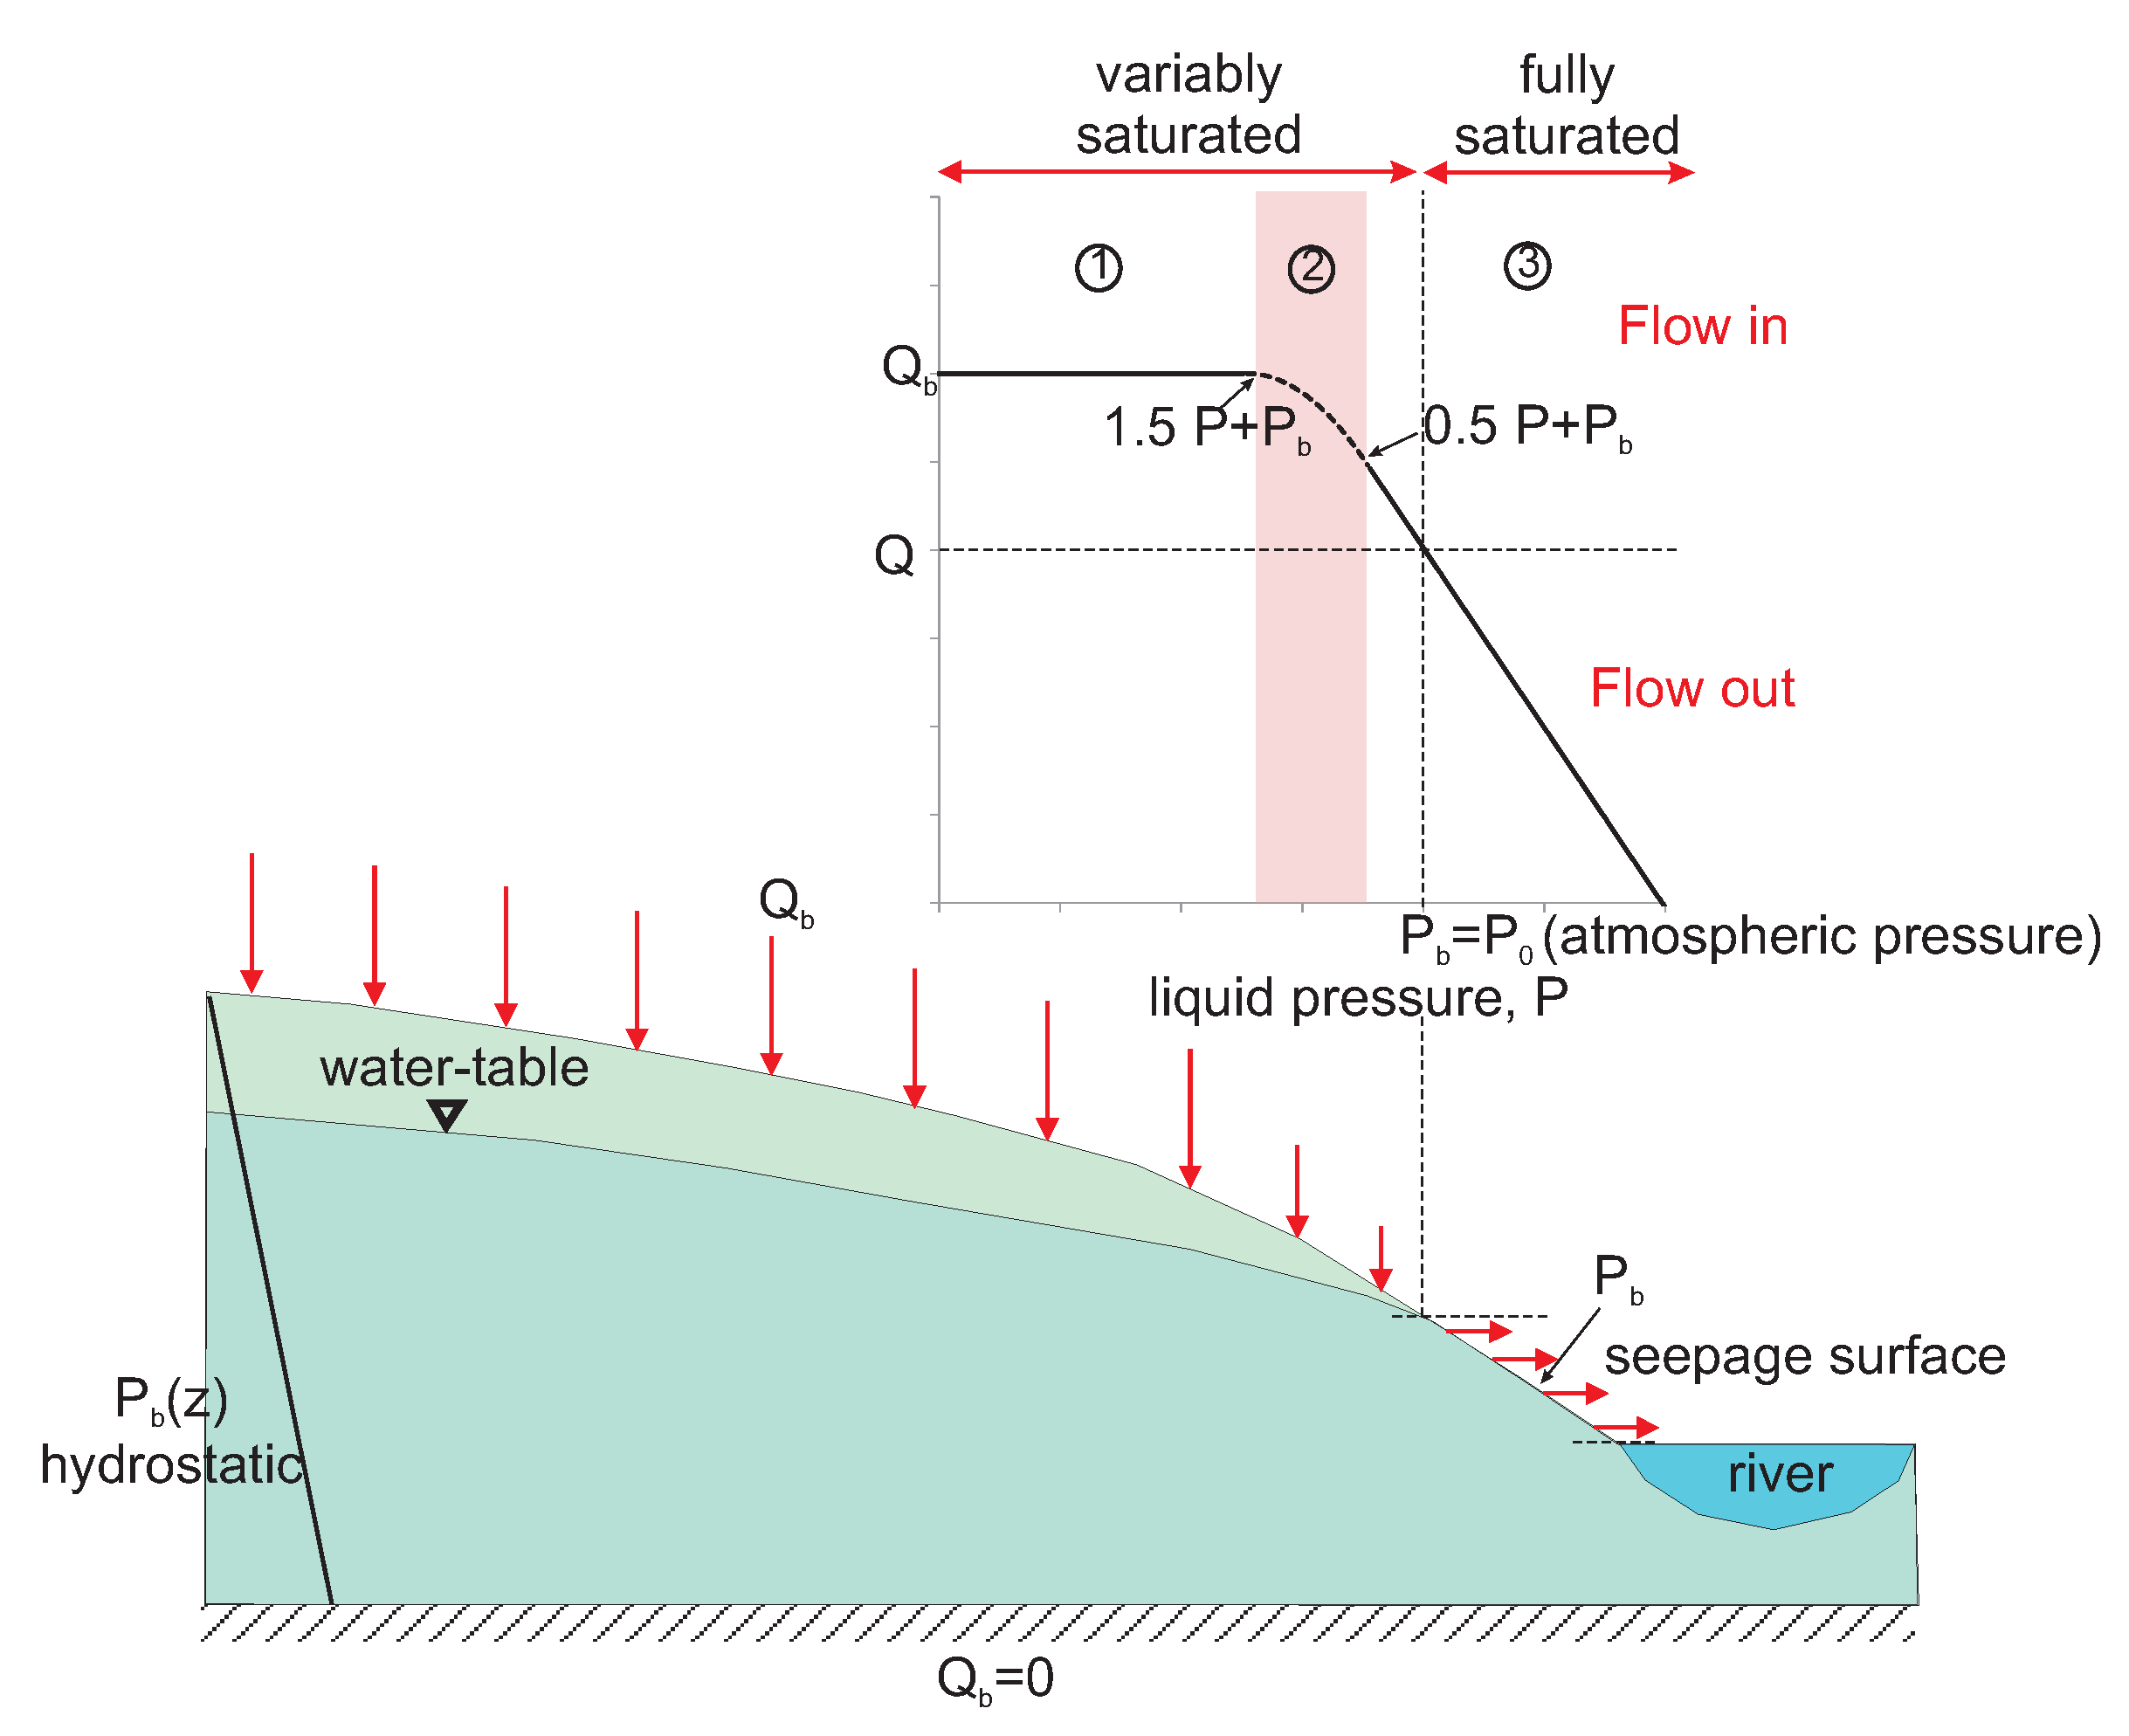
\includegraphics[scale=0.3]{seepage_bc.pdf}
\caption{Seepage face.}
\label{fig:seepage_bc}
\end{center}
\end{figure}

The state of the first option depends on the pressure inside the computational domain.
Regarding the second option, this hybrid boundary condition \citep[based on][]{hamm2000} can be formulated as
\begin{equation} \label{eq:fifth_bc_richard}
\begin{array} {llll}
  \bq \cdot \bn & = & q_{b}(t) &  p < \left( \frac{3}{2} p' + p_{0} \right) \\[0.5ex]
  \bq \cdot \bn & = & \frac{\left(  7-2f-f^{2}  \right)}{8} q_{b}(t) 
                    & \left( \frac32 p' + p_{0} \right) \leq p \leq \left( \frac12 p' + p_{0} \right) \\[1.0ex]
  \bq \cdot \bn & = & I (p - p_{0}) & \left( \frac{1}{2} p' + p_{0} \right) < p 
\end{array} 
\end{equation}
where $q_{b}(t)$ is the maximum recharge and $f(p,t)$ is a local variable between $-1$ and $1$ 
defined as 
\begin{equation}
  f(p,t) = 2 \frac{p'- (p(x_{b},y_{b},z_{b},t) - p_{0}) }{p'}
\end{equation}
where $p_{0}$ is a reference pressure (in this particular example case, its value is equal to 
the atmospheric pressure), and $p'$ is defined as 
\begin{equation}
  p' = I^{-1} q_{b}(t).
\end{equation}

